%%
%% This is file `sample-sigconf-authordraft.tex',
%% generated with the docstrip utility.
%%
%% The original source files were:
%%
%% samples.dtx  (with options: `all,proceedings,bibtex,authordraft')
%% 
%% IMPORTANT NOTICE:
%% 
%% For the copyright see the source file.
%% 
%% Any modified versions of this file must be renamed
%% with new filenames distinct from sample-sigconf-authordraft.tex.
%% 
%% For distribution of the original source see the terms
%% for copying and modification in the file samples.dtx.
%% 
%% This generated file may be distributed as long as the
%% original source files, as listed above, are part of the
%% same distribution. (The sources need not necessarily be
%% in the same archive or directory.)
%%
%%
%% Commands for TeXCount
%TC:macro \cite [option:text,text]
%TC:macro \citep [option:text,text]
%TC:macro \citet [option:text,text]
%TC:envir table 0 1
%TC:envir table* 0 1
%TC:envir tabular [ignore] word
%TC:envir displaymath 0 word
%TC:envir math 0 word
%TC:envir comment 0 0
%%
%%
%% The first command in your LaTeX source must be the \documentclass
%% command.
%%
%% For submission and review of your manuscript please change the
%% command to \documentclass[manuscript, screen, review]{acmart}.
%%
%% When submitting camera ready or to TAPS, please change the command
%% to \documentclass[sigconf]{acmart} or whichever template is required
%% for your publication.
%%
%%
\documentclass[sigconf,nonacm]{acmart}

\usepackage{titlesec}

% Redefine subsubsection to always start a new line
\titleformat{\subsubsection}[block]
  {\normalfont\normalsize\bfseries}
  {\thesubsubsection}{1em}{}


\usepackage{enumitem} % Package for customizing lists

\setlist[enumerate,1]{label=\arabic*., leftmargin=1em, itemsep=0.75em} % Outer list customization
\setlist[enumerate,2]{label=\alph*., leftmargin=2em, itemsep=0.25em} % Inner list customization


% Load the fancyhdr package
\usepackage{fancyhdr}

% Disable ACM headers and footers
\settopmatter{printacmref=false, printfolios=false}

\fancyhead[L]{\shorttitle} % Left-aligned: Document title
\fancyhead[R]{\shortauthors} % Right-aligned: Author's short name


%%
%% \BibTeX command to typeset BibTeX logo in the docs
\AtBeginDocument{%
  \providecommand\BibTeX{{%
    Bib\TeX}}}


%%
%% Submission ID.
%% Use this when submitting an article to a sponsored event. You'll
%% receive a unique submission ID from the organizers
%% of the event, and this ID should be used as the parameter to this command.
%%\acmSubmissionID{123-A56-BU3}

%%
%% For managing citations, it is recommended to use bibliography
%% files in BibTeX format.
%%
%% You can then either use BibTeX with the ACM-Reference-Format style,
%% or BibLaTeX with the acmnumeric or acmauthoryear sytles, that include
%% support for advanced citation of software artefact from the
%% biblatex-software package, also separately available on CTAN.
%%
%% Look at the sample-*-biblatex.tex files for templates showcasing
%% the biblatex styles.
%%

%%
%% The majority of ACM publications use numbered citations and
%% references.  The command \citestyle{authoryear} switches to the
%% "author year" style.
%%
%% If you are preparing content for an event
%% sponsored by ACM SIGGRAPH, you must use the "author year" style of
%% citations and references.
%% Uncommenting
%% the next command will enable that style.
%%\citestyle{acmauthoryear}


%%
%% end of the preamble, start of the body of the document source.
\begin{document}

%%
%% The "title" command has an optional parameter,
%% allowing the author to define a "short title" to be used in page headers.
\title{Professor Insights: Clustering Quality and Difficulty Across NCSU Colleges}

%%
%% The "author" command and its associated commands are used to define
%% the authors and their affiliations.
%% Of note is the shared affiliation of the first two authors, and the
%% "authornote" and "authornotemark" commands
%% used to denote shared contribution to the research.
\author{Nathaniel Lorenc}
\affiliation{%
  \institution{North Carolina State University}
  \city{Raleigh}
  \state{North Carolina}
  \country{USA}
}
\email{ndlorenc@ncsu.edu}

\author{Christopher Elchik}
\affiliation{%
  \institution{North Carolina State University}
  \city{Raleigh}
  \country{North Carolina, USA}
}
\email{cwelchik@ncsu.edu}

\author{Rishi Jeswani}
\affiliation{%
  \institution{North Carolina State University}
  \city{Raleigh}
  \country{North Carolina, USA}
}
\email{rjeswan2@ncsu.edu}

\author{Brandon Troy}
\affiliation{%
  \institution{North Carolina State University}
  \city{Raleigh}
  \country{North Carolina, USA}
}
\email{bjtroy@ncsu.edu}

%%
%% By default, the full list of authors will be used in the page
%% headers. Often, this list is too long, and will overlap
%% other information printed in the page headers. This command allows
%% the author to define a more concise list
%% of authors' names for this purpose.
\renewcommand{\shortauthors}{Lorenc et al.}

%%
%% The abstract is a short summary of the work to be presented in the
%% article.
\begin{abstract}
  This paper explores patterns in professor quality and difficulty ratings across colleges at North Carolina State University (NCSU). Using data aggregated from RateMyProfessor and NCSU Gradient, we applied clustering techniques to examine similarities and differences in teaching trends across colleges. The dataset combines metrics such as teaching quality, course difficulty, and GPA, processed through fuzzy-matching and normalization methods. After evaluating multiple clustering algorithms, K-Means was selected for its computational efficiency and interpretability. This resulted in distinct groupings of professors—such as high-quality with low difficulty and low-quality with high difficulty—providing insight into student experiences across disciplines. These findings answer debates about inter-college teaching quality, offering a data-driven perspective for academic decision-making.
\end{abstract}
\maketitle

\section{Background}

\subsection{Problem}
Many students, such as ourselves, use professor reviews to help guide course enrollment decisions, using sites such as RateMyProfessor. However, it is unclear how much contextual factors and personal biases affect these ratings. As a result, comparing professor quality, particularly across different departments, is challenging, and is likely often driven by stereotypes more than objective reasoning.

Additionally, NCSU undergraduate students have long debated over which college has it better or worse with regard to professors overall. This paper aims to provide insight into this question with a data-driven response. The specific question we will discuss is, \textit{How similar or dissimilar are different colleges (within NCSU) by professor quality and difficulty?}

While exploring this question, the specific refinements we utilized include optimizing and evaluating multiple clustering algorithms on our input data using techniques such as GridSearchCV and silhouette scoring. Some special cases we addressed were handling missing data (professors in one data source but not the other), non-standardized data (professor names with different spelling / formatting), and outliers like colleges that only had a handful of professors.

\subsection{Related Work}
To contextualize this problem, we wanted to find out what typically goes into professor reviews from the student's perspective. In \cite{10.3389/feduc.2022.842640:sourceD} a student survey was conducted and 75\% of the responses indicated that “assessment policies and practices,” “personality,” and “pedagogical knowledge” were the most important qualities in a professor. The same study found that student-professor rapport was one of the strongest predictors of professor ratings, accounting for 54\% of the variability in a sample of ratings.

On a more macroscopic level, we also looked at a paper that discussed typical aggregate trends in professor rating distributions. The paper noted that ratings distributions are usually left-skewed, with the majority of ratings being positive but few negative ratings shifting the mean below the median. In regards to the correlation between ratings and outcomes, they stated, “[Research] demonstrated a low to moderate positive correlation between students’ ratings and their grades or expected grades” \cite{LINSE201794:sourceE}.

We also researched clustering methods commonly used in machine learning applications to help guide our experiment procedures. Sources \cite{Abbas2005:sourceA} and \cite{Xu2015:sourceC}, gave a higher-level overview of multiple algorithms, including their typical behaviors and the pros and cons of each. Both discuss the K-means algorithm, and mention its efficiency, and sensitivity to noise and cluster count, making parameter tuning very important. Additionally, we found a more data-oriented paper, \cite{10.1371/journal.pone.0210236:sourceB} which compared metrics of multiple algorithms across experiments with a variety of input data. Its results generally agreed with the other two papers, and it additionally noted that K-means doesn't do particularly well in non-convex cases or when the scale of the clusters differs greatly. It is worth noting that they used the R implementations of the algorithms, while we are using Sci-kit Learn in Python, but the results likely generalize across implementations for the most part. These papers helped guide our selection of algorithms to test before selecting the one that performed the best with our data.

\section{Methods}

\subsection{Novel Aspects}
To address the novelty requirements, we created/transformed a custom dataset and used pattern-finding techniques to create new knowledge.

Our final dataset consisted of information scraped from multiple sources for 2681 professors (see 3.1 Datasets for specifics). To compile this dataset, we scraped all RateMyProfessor data for NCSU professors, as well as the Gradient grade distribution data for all undergraduate class sections.

After collecting the raw data, we applied transformations to aggregate and reformat the data such that machine learning techniques can be used. We used fuzzy search to cross-reference professors from RateMyProfessor and Gradient to account for slight name variations (i.e., Roman numerals, 'PhD', shortened names, etc.) and aggregated all relevant data from both sources into a single .csv file. We converted the Gradient data from a list of classes each with a map containing how many students received each letter grade to a GPA average for each class, then combined those with a weighted average for each professor.

Our data collection addresses the novelty requirement because we utilized web scraping techniques to collect raw data that was not immediately appropriate for machine learning tasks (raw .json data). We then transformed the data into a .csv file specifically formatted to be converted to a pandas dataframe, which is friendly for machine learning.

An additional item of novelty, as described by the project description, is that we used analytics and pattern-finding algorithms to create new knowledge. After creating our dataset, we applied clustering algorithms and analyzed the nature and composition of the clusters, ultimately providing new, data-driven insight into the similarities/differences in difficulty of professors between NCSU colleges. (See 2.2 Approach for algorithm specifics.)

\subsection{Approach}
In performing machine learning on our collected data in search of insight toward our main question, we first began by evaluating various clustering algorithms. We performed hyper-parameter grid search tuning on each of the clustering algorithms we evaluated, using the entire dataset of professors. We tested Spectral Clustering, Affinity Propagation, K-Means, Mini-Batch K-Means, Agglomerative, and Gaussian Mixtures clustering algorithms. For each of these clustering algorithms, we created both a 2D and 3D graph to visualize the clusters made by each algorithm to visually compare the separation provided by each.

From our visual inspection of each clustering graph, we concluded that the K-Means clustering algorithm provided the most separation between clusters. As such, we used the K-Means clustering algorithm for performing clustering on the professor data for each college individually using the hyper-parameters found during hyper-parameter grid search tuning previously. Lastly, we created 2D and 3D graphs for the clustering of each college's professor dataset.

\subsection{Rationale}
We decided to use clustering as an unsupervised learning approach since it allows us to reveal patterns without the need for predefined labels. Clustering is very well-suited for our situation, as we are specifically trying to group professors based on difficulty and quality ratings, where we can compare these groups between different colleges to analyze the statistical similarities and differences. Thus, these clusters can be used to provide insight into student experiences with professors across different NCSU colleges.

After performing experiments with different clustering algorithms (in clustering\textunderscore{}eval.ipynb), we decided to use K-Means clustering. K-Means performed the best in terms of computational efficiency, partition quality, and overall simplicity, as it scaled effectively to our large dataset. K-Means also produced the highest quality visualizations with its partitions, as shown in the plots below.

% \begin{figure}[h]
%     \centering
%     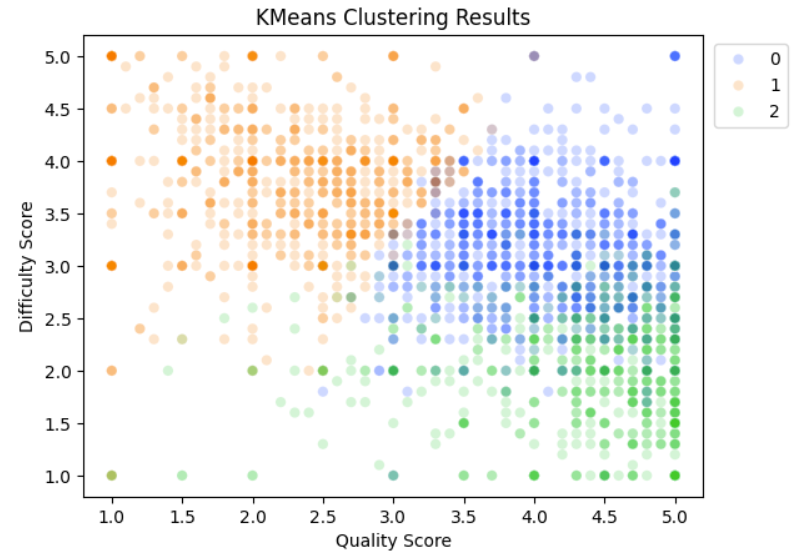
\includegraphics[width=0.5\linewidth]{Screenshot 2024-11-19 175849.png}
%     \caption{K-Means Clustering Visualization on Entire Dataset}
%     \label{fig:enter-label}
% \end{figure}

\begin{figure}[h]
    \centering
    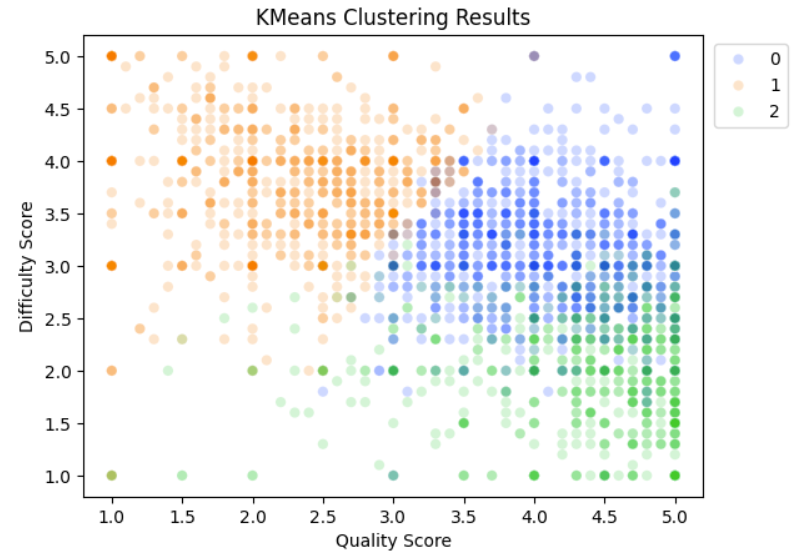
\includegraphics[width=0.45\linewidth]{Screenshot 2024-11-19 175849.png}
    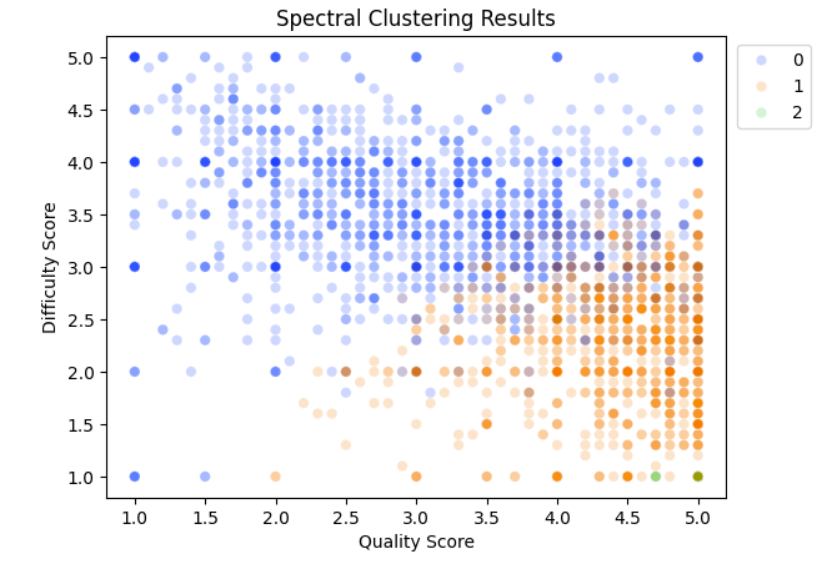
\includegraphics[width=0.45\linewidth]{spectral_clustering_results.png}
    \caption{K-Means (left) and Spectral Clustering (right) Visualizations on Entire Dataset}
    \label{fig:enter-label}
\end{figure}

K-Means clustering outperformed Spectral Clustering, in this case, as K-Means better produced more interpretable, meaningful clusters that could be analyzed, as shown by the heavily unbalanced result of Spectral Clustering (where cluster 2 is hardly noticeable in the bottom right). 

Other algorithms that we tested included Agglomerative Clustering, Gaussian Mixtures, and Affinity Propagation. Agglomerative Clustering was unable to scale well to our large dataset, as it did not produce clear, fixed partitions. Gaussian Mixtures inherently assumes the data exhibits a Gaussian distribution, which was not quite fitting for our dataset. Affinity Propagation, due to its ability to tune the number of clusters, resulted in an uninterpretable plot with 77 different clusters, which is less useful than K-Means with a set hyperparameter of 3 clusters. (For the other visualizations, see clustering\textunderscore{}eval.ipynb in the Team 8 repository.)

An important simplification we made was choosing 3 clusters for the K-Means clustering. Though this simplification was decided using the elbow method and silhouette scoring (via GridSearchCV), using 3 clusters also allows us to analyze 3 groups of professors within each college: high quality with low difficulty, high quality with high difficulty, and low quality with high difficulty. This aligns with the sparsity of low-quality with low-difficulty professors in our dataset, as seen in the above visualizations.

We opted to not attempt to examine any causality or use predictive models. Our goal in this research was purely exploratory, to find patterns in the difficulty and quality of professors across NCSU colleges. The insights we derive from clustering best support this goal, and our decision of K-Means resulted in the highest computational efficiency and visualization interpretability.

\section{Plan \& Experiment}
\subsection{Datasets}
The dataset for our project is custom-built through web scraping and combines data from RateMyProfessor and NCSU Gradient. It provides an extensive view of professor quality and difficulty ratings, as well as additional academic metrics, for all professors who taught at North Carolina State University (NCSU) during a recent semester. Below is the description of the dataset we used in detail, highlighting the features that enable our clustering analysis and pattern exploration.

\subsubsection{Features in the Dataset}

\begin{enumerate}
\item Professor Name
\begin{enumerate}
    \item Includes both first and last names of each professor.
    \item Source: RateMyProfessor and the NCSU Course Catalog.
\end{enumerate}
\item College
\begin{enumerate}
    \item Categorizes professors into one of the nine colleges at NCSU:  
College of Engineering, College of Sciences, College of Education,
    etc.  
    \item Source: NCSU Course Catalog.
\end{enumerate}
\item Quality Score
\begin{enumerate}
    \item A numerical score between 1 and 5, representing the average teaching quality as rated by students. 
    \item Source: RateMyProfessor.
\end{enumerate}
\item Difficulty Score
\begin{enumerate}
    \item A numerical score between 1 and 5, representing the perceived difficulty of the professor’s courses, as rated by students.  
    \item Source: RateMyProfessor.
\end{enumerate}
\item GPA
\begin{enumerate}
    \item The average grade (on a 4.0 scale) received by students in the professor’s courses.  
    \item Source: NCSU Gradient.
\end{enumerate}
\item Would Take Again
\begin{enumerate}
    \item The percentage of students who would choose to take this professor’s course again. 
    \item Source: RateMyProfessor.
\end{enumerate}
\item Number of Ratings
\begin{enumerate}
    \item The total number of student reviews submitted for the professor on RateMyProfessor.  
    \item Source: RateMyProfessor.
\end{enumerate}
\item Number of Sections
\begin{enumerate}
    \item The total number of sections the professor has taught during the semester in question.  
     \item Source: NCSU Gradient.
 \end{enumerate}
 \item Total Students
 \begin{enumerate}
     \item The total number of students taught by the professor across all sections.
     \item Source: NCSU Gradient.
 \end{enumerate}
\end{enumerate}



\subsubsection{Data Collection and Validation}

To construct the dataset, we began by scraping the NCSU Course Catalog to obtain a comprehensive list of professors and their associated colleges. Next, we utilized the RateMyProfessor API to gather ratings and feedback data, ensuring consistency and accuracy throughout the data collection process. Additionally, for course-specific metrics such as GPA, the number of sections, and total students, we relied on data from Gradient, a repository of course data available to students at NCSU.


\subsubsection{Relevance and Impact}

This dataset provides a robust foundation for exploring clustering patterns of professor quality and difficulty across NCSU colleges. By incorporating diverse attributes such as quality, difficulty, and GPA, alongside contextual information like college affiliation and teaching load, the dataset enables a multidimensional analysis of teaching trends. The inclusion of features like the "Would Take Again" percentage and number of ratings ensures that the dataset captures both quantitative metrics and student sentiment.

\subsubsection{Summary Statistics}

Before proceeding with clustering, the dataset will undergo pre-processing to handle missing or inconsistent data points, ensuring the validity of the results. Initial statistics, such as the distribution of ratings and GPA across colleges, will guide the analysis and highlight potential patterns.


\subsection{Hypotheses}
For our cluster analysis of professors at NCSU colleges, we have two main hypotheses. First, we hypothesize that there will be rather large densities of professors in the following two groups: high quality, low difficulty and low quality, high difficulty. Second, we hypothesize that the colleges with the most ratings will tend to have less defined clusters, leaning more towards an 'arc' trend with a negative correlation between quality and difficulty. This leads us to our overall question: \textit{How similar or dissimilar are different colleges (within NCSU) by professor quality and difficulty?}

\subsection{Experimental Design}
To test both hypotheses, we designed a comprehensive series of experiments leveraging clustering analysis on professor data across various colleges at NCSU. These experiments were structured to extract meaningful insights about trends in professor quality and difficulty, with results interpreted differently to address each hypothesis.

\subsubsection{Data Pre-processing}
The first step involved web scraping data from two primary sources: RateMyProfessor and NCSU Gradient. RateMyProfessor provided ratings and feedback, while NCSU Gradient offered course-specific metrics like GPA, the number of sections taught, and total enrollment. Data collection posed significant challenges, including the need for authorization and the complexity of reverse-engineering some sources. Although we initially relied on a minimal open-source library for RateMyProfessor, its limitations (e.g., name-based searches capped at eight results per query) prompted us to reverse-engineer the GraphQL requests made by the browser instead. This approach allowed us to increase the query limit to 2,000 results per request, enhancing efficiency by approximately 400-fold. For NCSU Gradient, which requires Unity ID authentication, we included authorization headers and implemented significant rate-limiting to avoid overloading the server.

Integrating data from these sources introduced additional challenges, such as variations in professor names due to differences in order, middle names, or abbreviations. To address this, we used fuzzy matching techniques to cross-reference and standardize names, ensuring consistency between datasets. Professors with incomplete or missing data were excluded to maintain reliability, and by limiting the dataset to professors present in both sources, we naturally filtered outliers such as individuals who had not taught recently or lacked ratings. The refined dataset, upon review, did not exhibit any significant outliers that skewed clustering results, providing a solid foundation for extracting meaningful insights tailored to our hypotheses.

\subsubsection{Clustering Analysis}
The clustering analysis focused on three primary features: quality, difficulty, and GPA, representing key attributes of professor performance and student experience. Selecting the most suitable clustering algorithm was a significant challenge, as each algorithm had strengths and limitations depending on the characteristics of the data. We initially explored advanced methods like Spectral Clustering and Gaussian Mixture Models for their ability to handle complex relationships and overlapping data points. However, these methods often introduced computational overhead and less interpretable results, making them less practical for our specific use case. Ultimately, we chose K-means due to its simplicity, efficiency, and ability to generate distinct and easily interpretable clusters, which aligned well with the goals of our analysis.

To ensure that K-means provided meaningful insights, we fine-tuned key hyperparameters, such as the number of clusters, using grid search to optimize performance. Visualizing the clustering results for each college allowed us to clearly see how professors grouped based on quality, difficulty, and GPA, highlighting patterns and distinctions across different colleges. Despite the initial challenges in selecting the algorithm, K-means proved to be an effective choice for uncovering trends in professor attributes at NCSU.

\subsubsection{Evaluation}
The evaluation phase focused on analyzing the characteristics of clusters within each college and comparing these results across colleges. For each cluster, we examined the centroids, which represented the average values of quality, difficulty, and GPA for professors within that group. These centroids provided a clear snapshot of trends within each cluster and were instrumental in assessing the density and distinctness of clusters. To uncover broader patterns, we compared clustering results across colleges by constructing both 2D and 3D plots, examining them from different perspectives. This allowed us to explore correlations, such as the hypothesized negative correlation 'arc' between quality and difficulty, and identify similarities in professor distributions across colleges. Particular attention was given to whether colleges exhibited well-defined clusters or more continuous trends.

During the evaluation process, we encountered challenges related to data integrity. Despite our algorithmic approach to matching professors across the datasets, there were a few cases with large name discrepancies that required manual adjustment. Additionally, data sparsity in smaller colleges posed a challenge, as limited information on professors could hinder the formation of meaningful clusters. This required meticulous handling to ensure fair representation while maintaining the accuracy and reliability of clustering outcomes. Despite these issues, the evaluation provided valuable insights into professor attributes and trends within and across colleges.


We used the same process for both hypotheses to ensure the results were consistent. The findings will either agree with or challenge our ideas and give us new insights into how professor quality, difficulty, and student outcomes are connected.


\section{Results}
The results of our experiment are plentiful since we are performing a cluster analysis of the professors of each college at NCSU. For each college, two graphs are provided: a 2D graph and a 3D graph. The majority of the analysis will be on the 2D graphs, given that these graphs show only the RateMyProfessor attributes as dimensions of the graph, however, both graphs use the Gradient GPA attribute when clustering was performed, and the 3D graph shows the impact GPA has on the clustering results better. Lastly, all clustering results have three clusters, but these clusters are determined by the data for each college.

\subsection{Observations}
\begin{figure}[H]
    \centering
    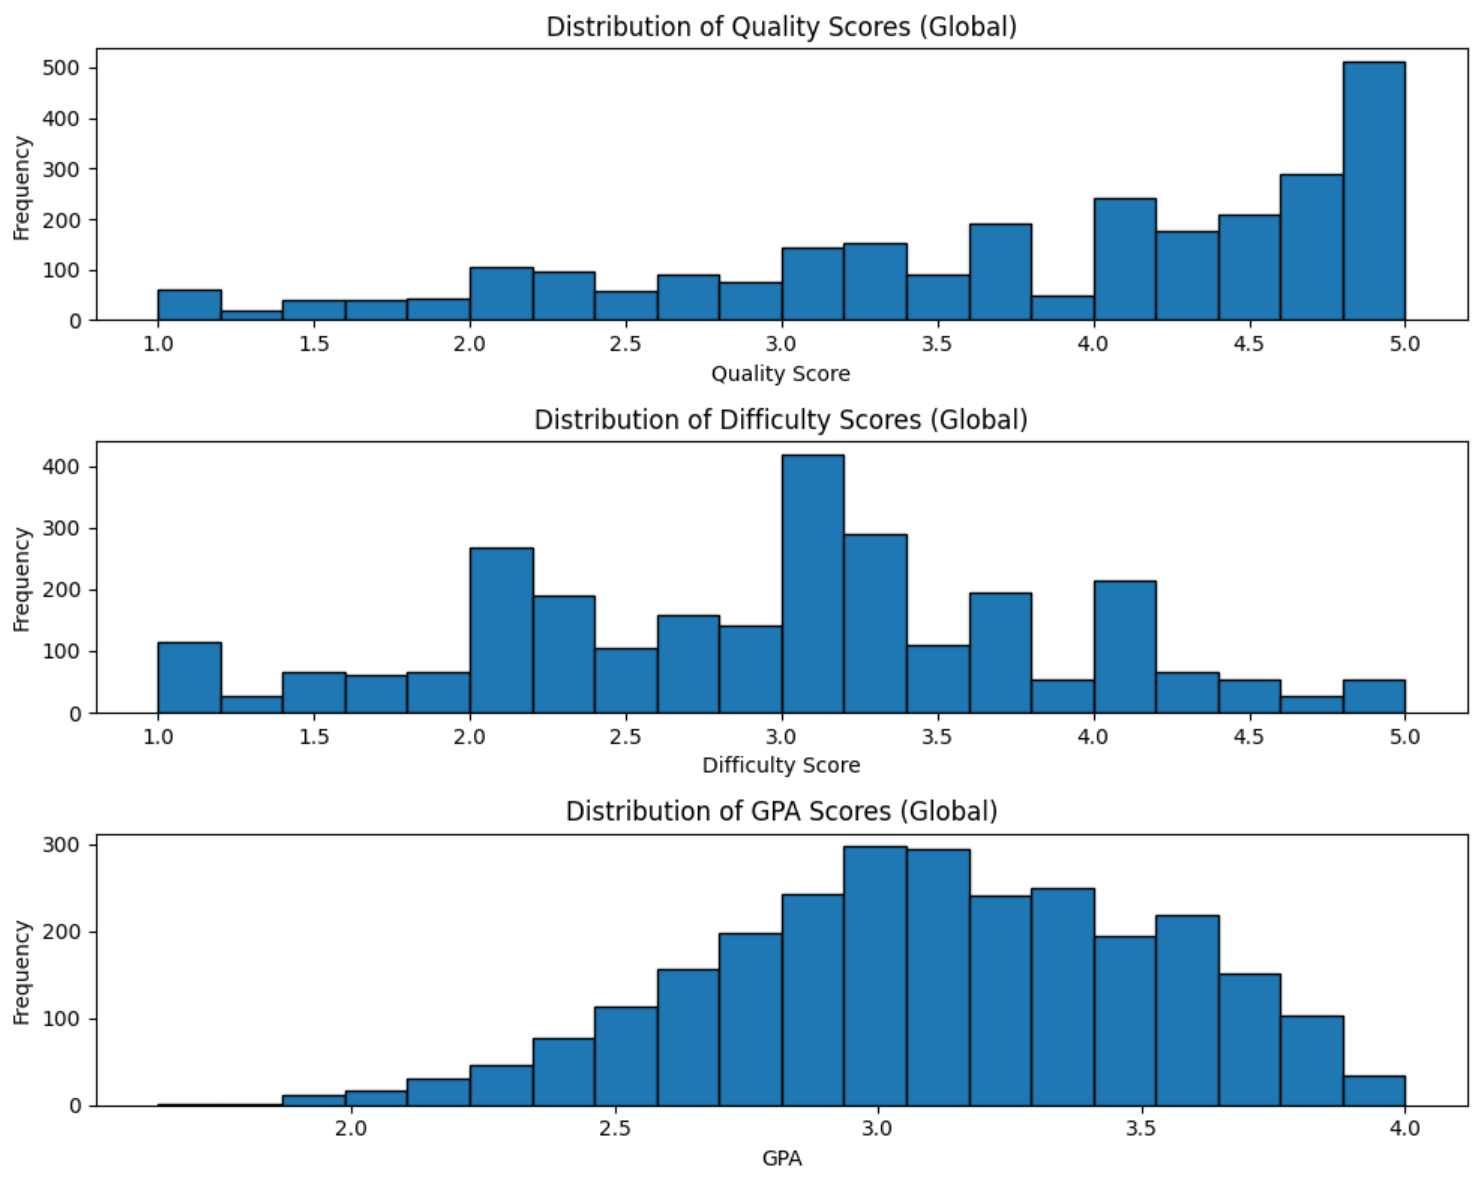
\includegraphics[width=0.9\linewidth]{images/aggregate-distributions.png}
    \label{fig:enter-label}
\end{figure}

One of the first things we did after generating our dataset was visualize the overall distribution of our three metrics. As you can see, the quality ratings distribution very strongly aligns with the remark from \cite{LINSE201794:sourceE} with regard to its skewness.

\begin{figure}[H]
    \centering
    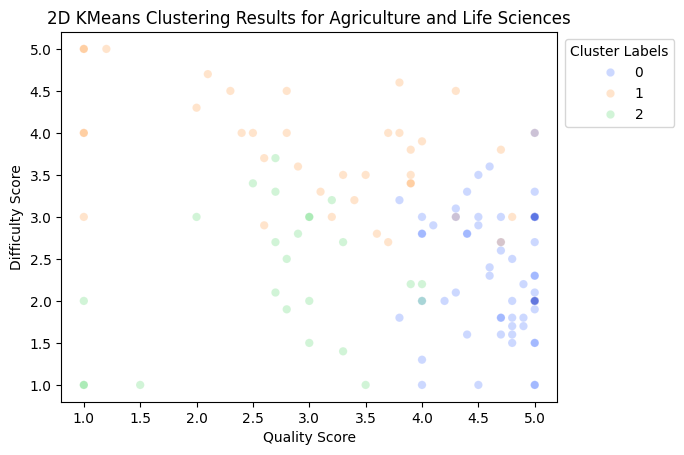
\includegraphics[width=0.45\linewidth]{images/agriculture-2d.png}
    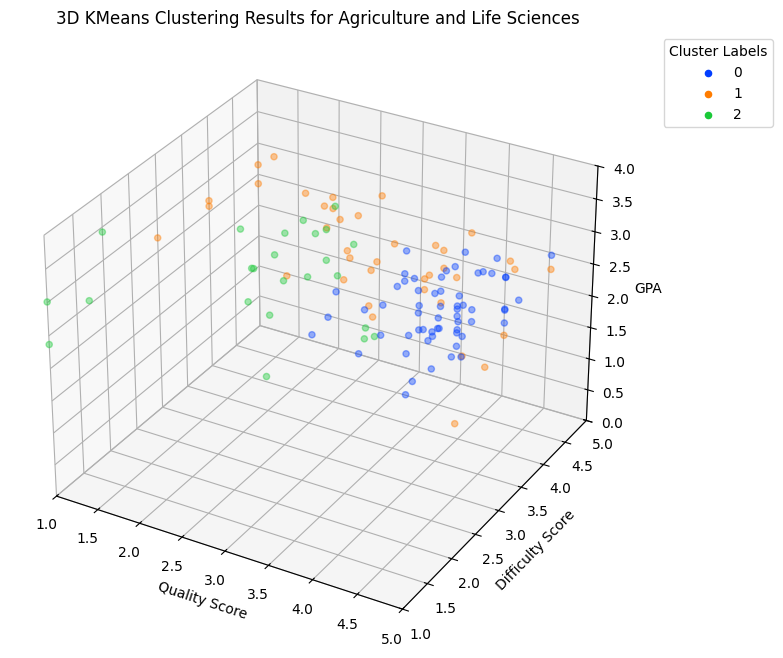
\includegraphics[width=0.45\linewidth]{images/agriculture-3d.png}
    \caption{College of Agriculture K-Means Clustering (left) 2D-Graph (right) 3D-Graph}
    \label{fig:enter-label}
\end{figure}

The College of Agriculture and Life Sciences has very distributed clusters, which is a result of the varied RateMyProfessor scores for the college. When looking at the 2D graph, the three clusters roughly span the bottom left quadrant, the bottom right quadrant, and the top half of the graph. GPA seems to somewhat affect the clustering, but most of the data is within a GPA of [2.0, 3.0] (C to B). The interesting note is that the few professors with low quality and difficulty scores have higher than average GPAs.

\begin{figure}[H]
    \centering
    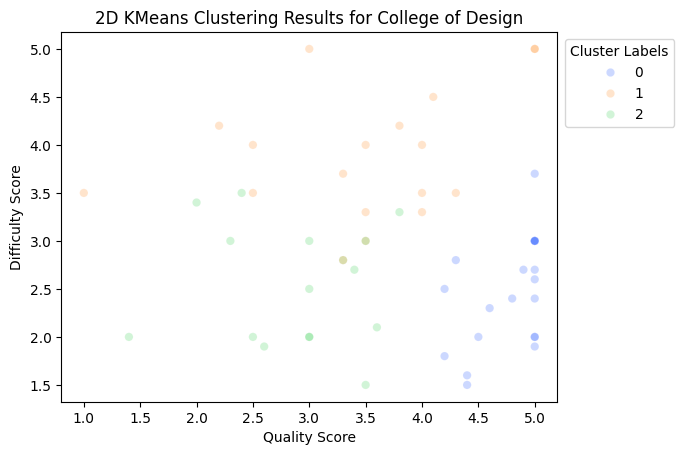
\includegraphics[width=0.45\linewidth]{images/design-2d.png}
    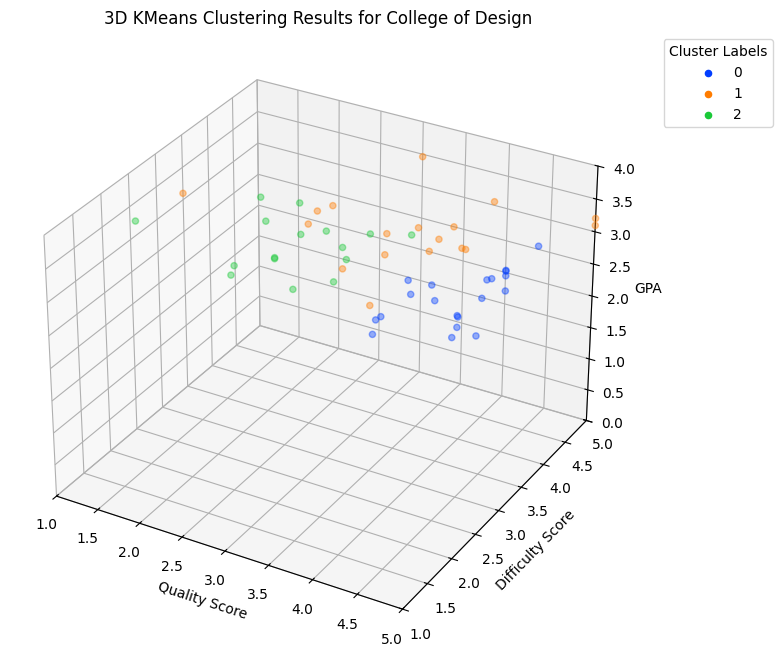
\includegraphics[width=0.45\linewidth]{images/design-3d.png}
    \caption{College of Design K-Means Clustering (left) 2D-Graph (right) 3D-Graph}
    \label{fig:enter-label}
\end{figure}

The College of Design mostly consists of professors with a quality score above 2.5. The clusters are split into: a relatively small section in the bottom right, the remaining bottom half, and the top half of the graph. The last two clusters are very spread out, with the low-quality professors almost being outliers. However, the small cluster in the bottom right has many professors with high-quality scores and relatively low difficulty. When including GPA in the discussion, that same small cluster also tends to have the highest GPAs out of all the collected professor data, with the other two clusters varying similarly.

\begin{figure}[H]
    \centering
    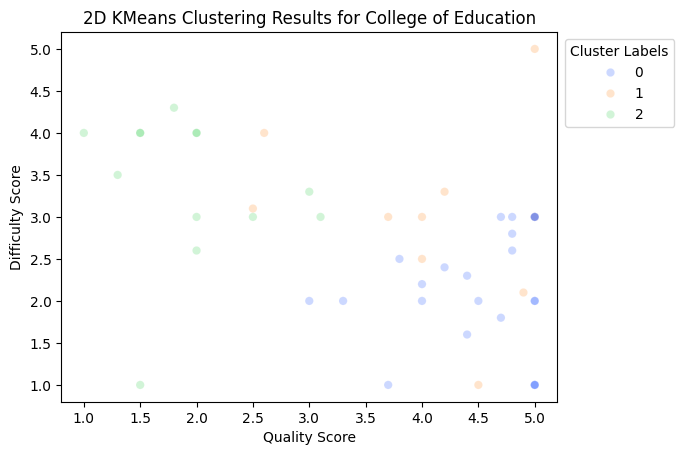
\includegraphics[width=0.45\linewidth]{images/education-2d.png}
    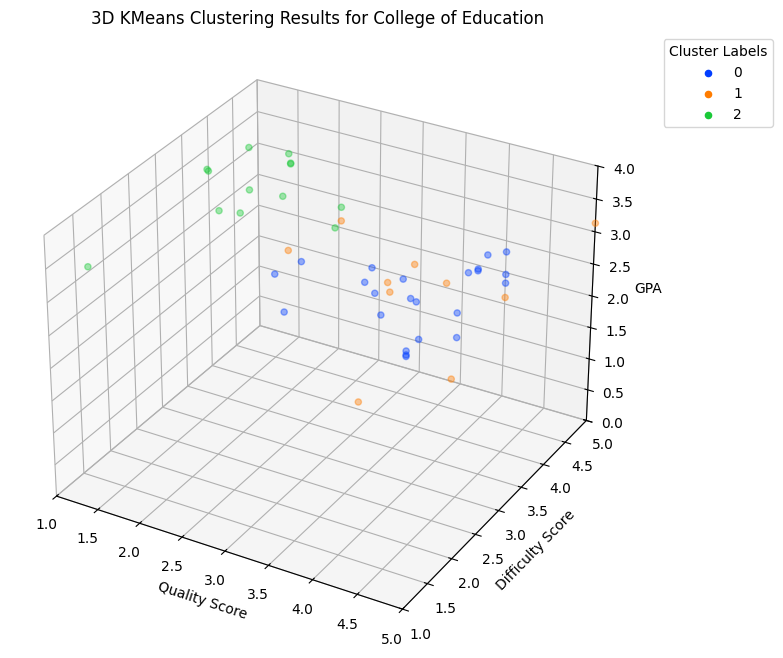
\includegraphics[width=0.45\linewidth]{images/education-3d.png}
    \caption{College of Education K-Means Clustering (left) 2D-Graph (right) 3D-Graph}
    \label{fig:enter-label}
\end{figure}

The College of Education doesn’t have an excessive number of professors. The professors tend to be within an arc, stretching from the top left corner to the bottom right corner of the 2D graph, with a width of about half of the graph. This results in three clusters: high-difficulty and low-quality professors, high-quality and low-difficulty professors, and a catch-all cluster that depends mostly on GPA. The catch-all cluster is a grouping of professors with significantly lower average GPAs as compared to the other two clusters, which are roughly equivalent to each other.

\begin{figure}[H]
    \centering
    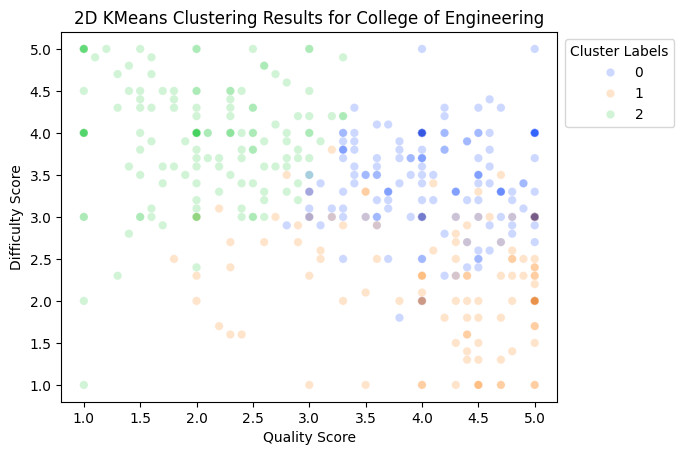
\includegraphics[width=0.45\linewidth]{images/engineering-2d.png}
    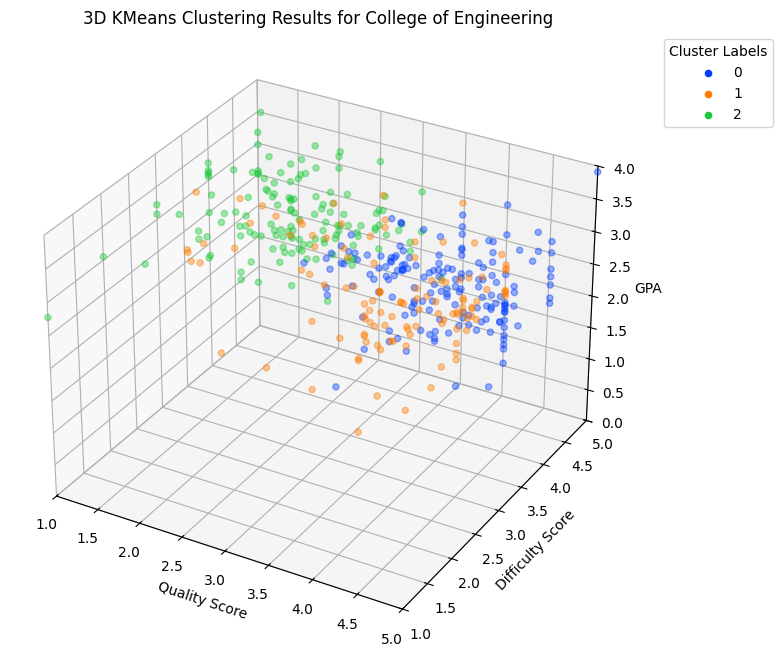
\includegraphics[width=0.45\linewidth]{images/engineering-3d.png}
    \caption{College of Engineering K-Means Clustering (left) 2D-Graph (right) 3D-Graph}
    \label{fig:enter-label}
\end{figure}

The College of Engineering contains a lot of professors, which helps the algorithm separate clusters out a bit better. There are three rather well-defined clusters: low-quality and high-difficulty professors, high-quality and low-difficulty professors, and high-quality and high-difficulty professors. This is the first college to have a significant number of well-liked, but also difficult, professors, so much so that there is a cluster for this combination, which is shown as cluster 0. While there is a cluster of professors that are well-liked and easy, the majority of the professors in the College of Engineering were found to be difficult, with clusters 0 and 2 depicting this.

\begin{figure}[H]
    \centering
    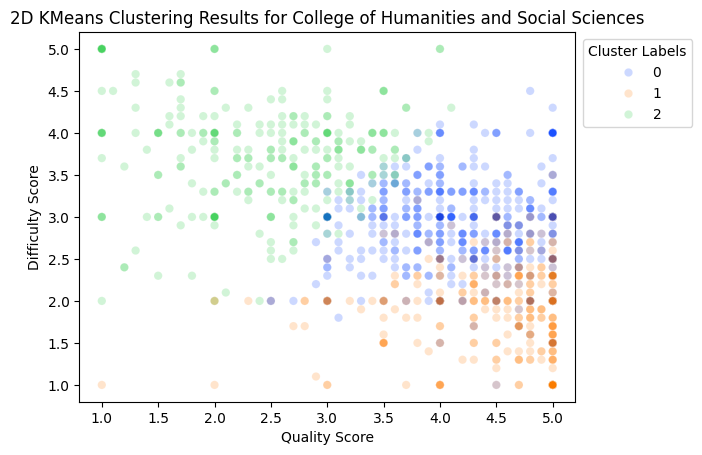
\includegraphics[width=0.45\linewidth]{images/humanities-2d.png}
    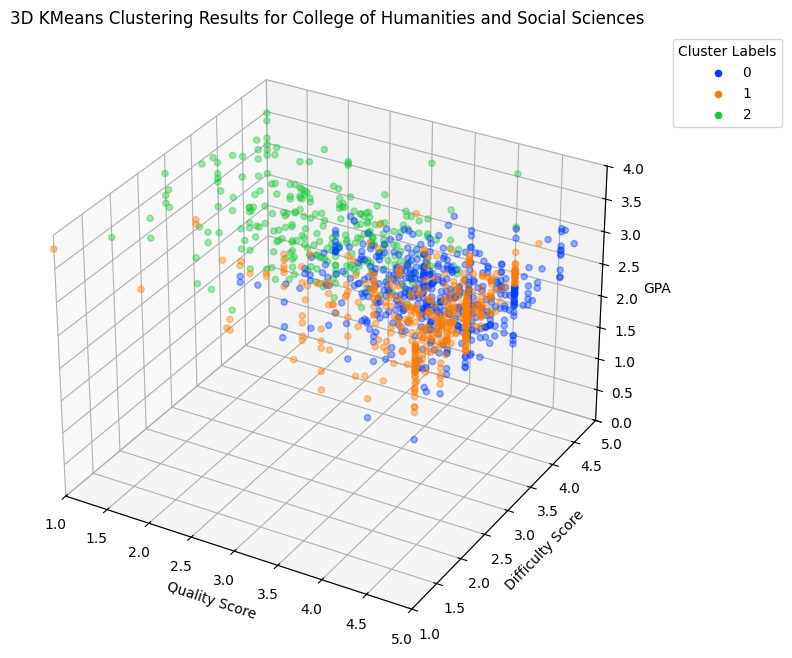
\includegraphics[width=0.45\linewidth]{images/humanities-3d.png}
    \caption{College of Humanities and Social Sciences K-Means Clustering (left) 2D-Graph (right) 3D-Graph}
    \label{fig:enter-label}
\end{figure}

The College of Humanities and Social Sciences is clustered similarly to the College of Engineering, but the difficulty for the clusters is lower. Cluster 1, while mostly toward the side of high quality, stretches across the quality spectrum while keeping with a low difficulty. Clusters 0 and 2 make up the remaining professors with cluster 0 having higher quality professors and cluster 2 having moderate to lower quality professors. Cluster 2 also includes some high-difficulty professors, with these points being rather far from the centroid.

\begin{figure}[H]
    \centering
    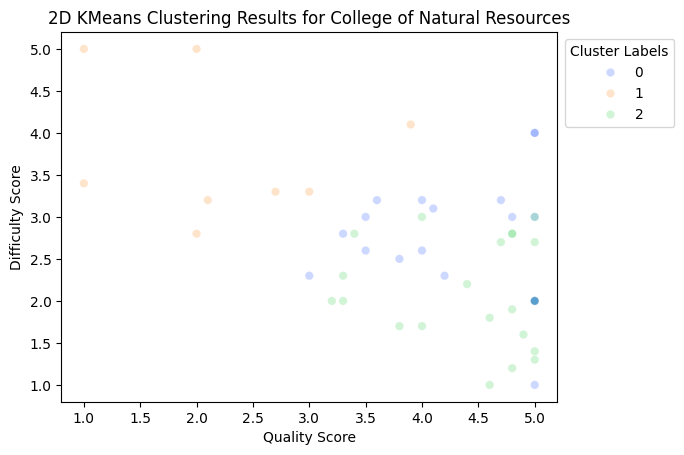
\includegraphics[width=0.45\linewidth]{images/natural-2d.png}
    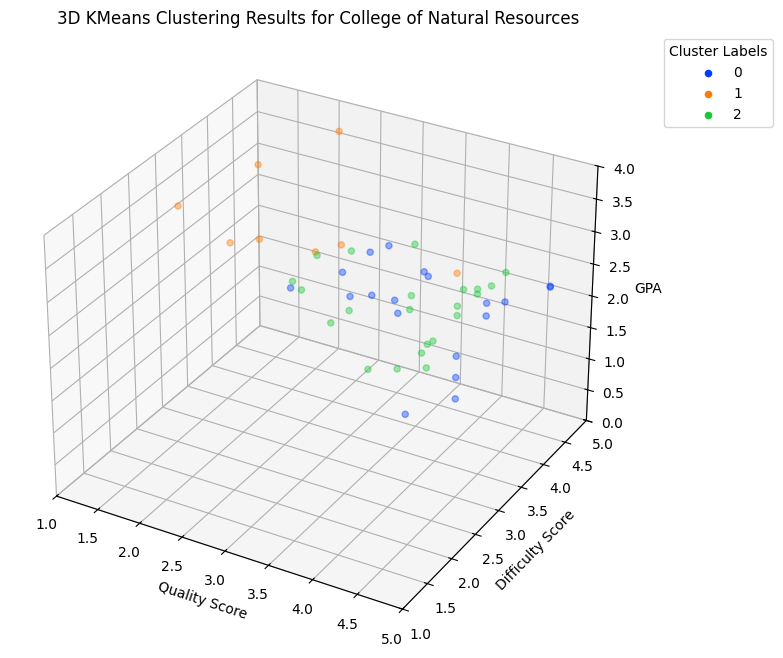
\includegraphics[width=0.45\linewidth]{images/natural-3d.png}
    \caption{College of Natural Resources K-Means Clustering (left) 2D-Graph (right) 3D-Graph}
    \label{fig:enter-label}
\end{figure}

The College of Natural Resources is small, but it appears to be large enough that professors can be clustered. As with most colleges, this college has a cluster of professors that maximize qualities students tend to look for: high quality, low difficulty, and high GPA. For this college in particular, not only does cluster 2 fit this well, but cluster 0 is also rather close. Cluster 1 contains the remaining professors that have lower quality or are more difficult, but the average GPA for most of these professors is still generally above 3.0.

\begin{figure}[H]
    \centering
    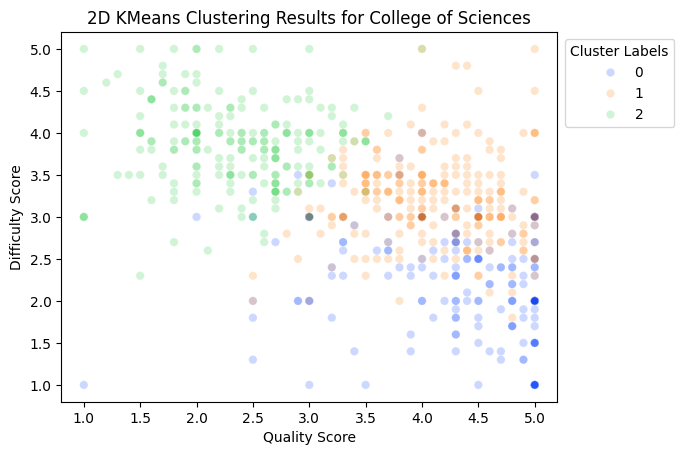
\includegraphics[width=0.45\linewidth]{images/sciences-2d.png}
    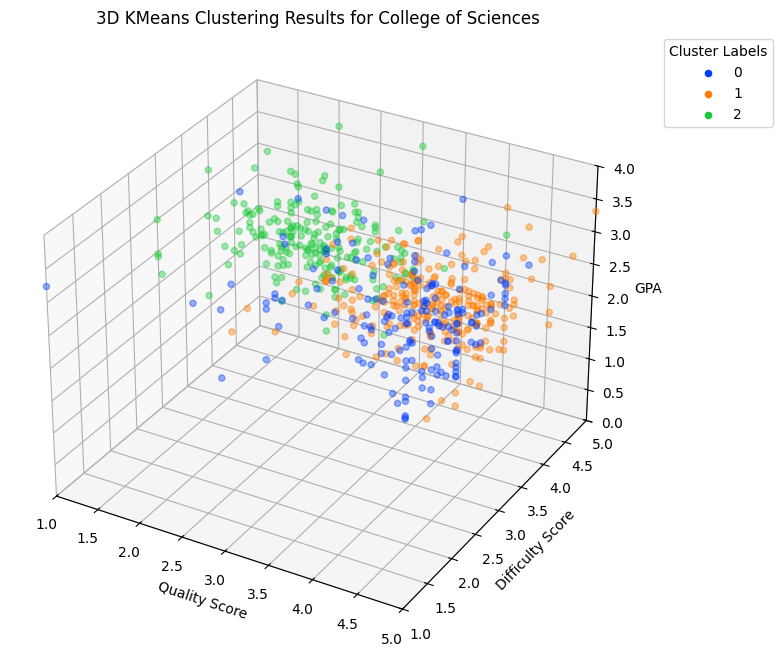
\includegraphics[width=0.45\linewidth]{images/sciences-3d.png}
    \caption{College of Sciences K-Means Clustering (left) 2D-Graph (right) 3D-Graph}
    \label{fig:enter-label}
\end{figure}

The College of Sciences has a higher-than-average number of professors. However, when looking at the clusters in the 3D graph, the clusters are more spread out than for other colleges. For those most concerned with a high GPA, cluster 0 generally contains professors with the highest GPAs. Cluster 0 also is in the bottom right corner of the 2D graph, high-quality and low-difficulty, which is generally appreciated by students. Clusters 1 and 2 have similar GPAs, but Cluster 1 tends to have higher-quality professors. In general, the professors for this college tend to not be above about 4.5.

\begin{figure}[H]
    \centering
    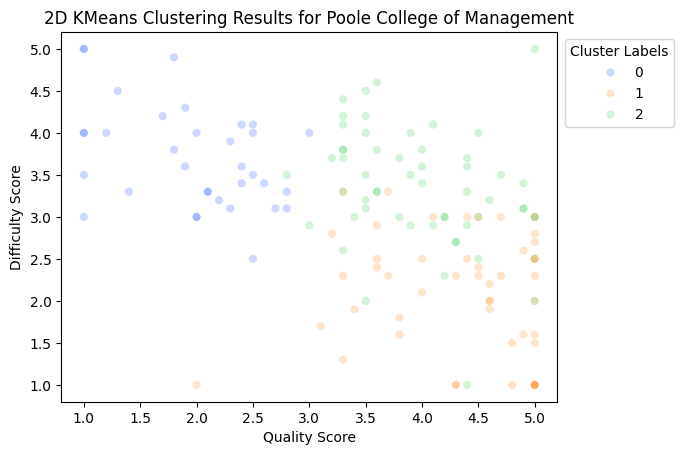
\includegraphics[width=0.45\linewidth]{images/poole-2d.png}
    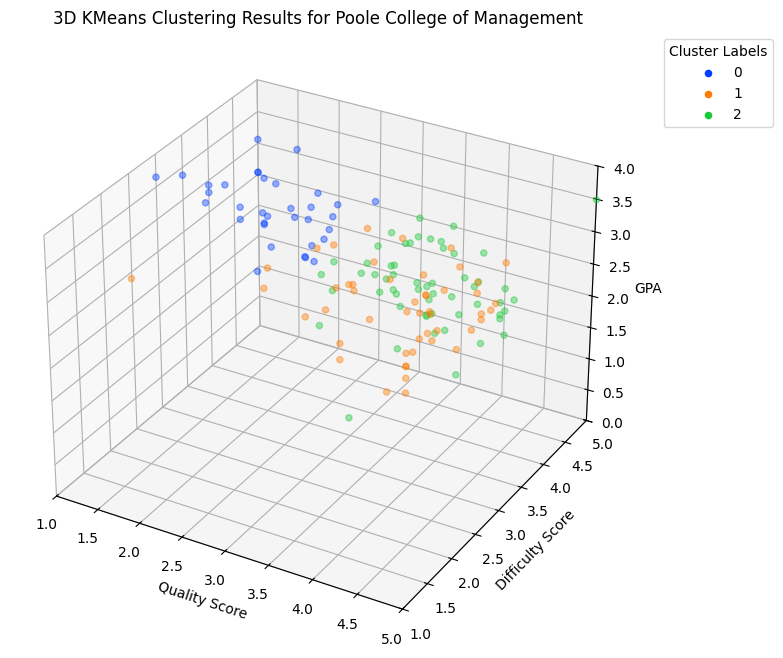
\includegraphics[width=0.45\linewidth]{images/poole-3d.png}
    \caption{Poole College of Management K-Means Clustering (left) 2D-Graph (right) 3D-Graph}
    \label{fig:enter-label}
\end{figure}

The Poole College of Management’s clusters of professors show an interesting trend. As a background, this college has three clusters that appear to fall into the first, second, and fourth quadrants rather well. This clustering is similar to other colleges but is more pronounced for this one in particular. More interestingly, clusters 0 and 1, clusters of extremes, have higher GPAs than cluster 2. While conventional interpretation would predict cluster 0 to have the lowest GPA due to high difficulty and low quality, the GPA is near that of the predictably high GPA for cluster 1. The data shows that choosing from one of the clusters of extremes is correlated with a higher GPA than the cluster of high-quality and difficult professors from who one would expect to learn the most.

\begin{figure}[H]
    \centering
    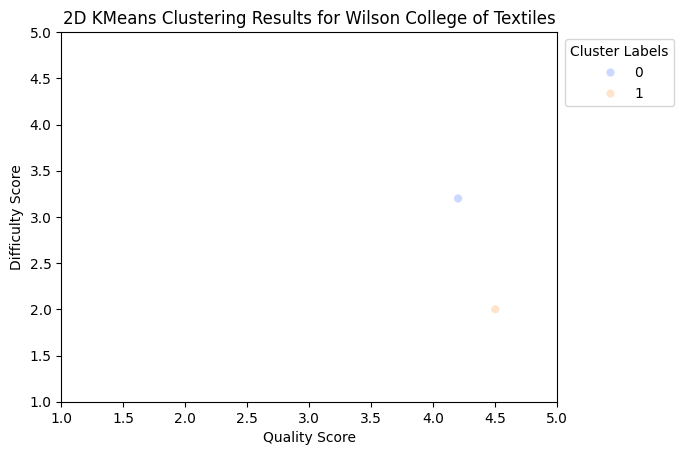
\includegraphics[width=0.45\linewidth]{images/textiles-2d.png}
    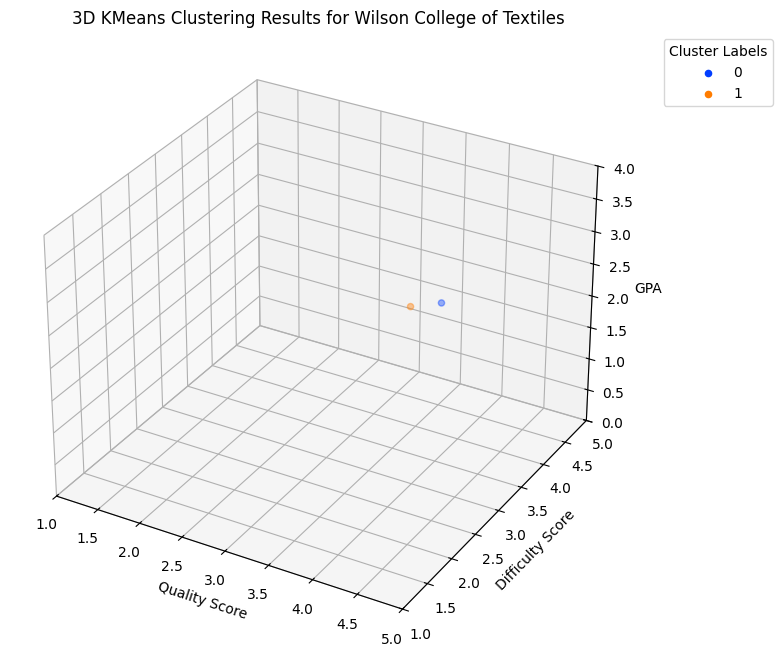
\includegraphics[width=0.45\linewidth]{images/textiles-3d.png}
    \caption{Wilson College of Textiles K-Means Clustering (left) 2D-Graph (right) 3D-Graph}
    \label{fig:enter-label}
\end{figure}

The College of Textiles resulted in a very limited number of professors that we matched among the RateMyProfessor and NCSU Gradient datasets. Since there are only two data points, the clustering result is insignificant and can be ignored. When the professor data is viewed, it shows that the professors in the College of Textiles are rather well-liked with moderate to low difficulty. This would put the two Textiles professors into the range of the better clusters as compared to other colleges, however, due to the very limited data points, this comparison can not be made.

\subsection{Discussion}

Some difficulties associated with the nature of this question are generalization and data consistency/quality. There will inherently be some survey bias because the ratings are on a volunteer basis. Also as a result of that, some professors may have no or very few ratings recorded, making it difficult to provide a complete representation of professors at NCSU. Additionally, our results are not necessarily directly applicable to other universities because our data solely included professors at NCSU. Lastly, we observed that contrary to popular belief, RateMyProfessor tends to include positive reviews of professors rather than act as a public avenue for disgruntled students.

Our hypotheses were generally correct, specifically for clustering in both (high quality, low difficulty) and (low quality, high difficulty) regions. The data also generally indicated a negative correlation between quality and difficulty and fell into an "arc" shape, with fewer points in the (low-quality, low-difficulty) or (high-quality, high-difficulty) quadrants. This pattern was visible in the aggregate plot, as well as for individual colleges with a substantial number of professors, further emphasizing that this pattern occurs as the number of professors increases.

Our experiment also showed that many preconceptions about the difficulty of coursework in various colleges are substantiated through responses of individuals within the respective college. For instance, the College of Engineering showed that professors in this college were particularly difficult, with two clusters comprised of professors with higher than average difficulties. However, there were a couple of surprises that were discovered within our experiment. First, the cluster in the Poole College of Management with highly rated professors and higher than average difficulties had the lowest GPAs by a significant margin. This is particularly troubling at an institution that is focused on learning because these results incentivize students to receive a lower-quality education in exchange for receiving a higher GPA. Second, our data suggests that students switching from more demanding majors to Business for a better experience could have been better off choosing a different college, namely the College of Natural Resources. With two clusters of professors being of high quality and low difficulty, the majority of professors a student could have in this college align well with the type of professor they want. Additionally, these two clusters of professors also tend to be associated with high GPAs. In conclusion, while many colleges had similar trends for professors, the Poole College of Management and the College of Natural Resources showed interesting deviations that should be investigated further.

\section{Conclusions}

In our research and testing, we learned a lot about different clustering algorithms, their traits, and how they can be evaluated. For example, we learned that K-Means and Spectral are very efficient, but sensitive to the number of clusters and proximity measure respectively. To further understand this data, we gained insights into the psychology behind professor reviews, what typical distributions look like, and how they can be interpreted. We had several ideas on how this project could be expanded upon that were out of the scope of the assignment. Firstly, we wanted to extract the contents of individual reviews and use language processing to categorize the contents into predetermined buckets (ie. policies, personality, knowledge, etc.), to determine the most common indicators of a positive rating. We could then compare the results with the findings of the papers we researched. Secondly, we could expand upon our dataset to include multiple institutions to determine if different school cultures affect noticeable trends in the data. This would help our findings generalize to universities across the country. With these two additions, the significance of our results could sharply increase.

\newpage

\section{Meeting Attendance}

\begin{figure}[H]
    \centering
    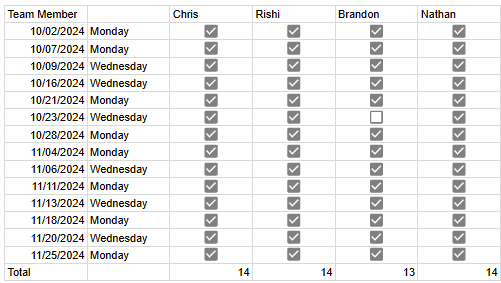
\includegraphics[width=1\linewidth]{updated_attendance.png}
    \caption{Meeting Attendance for Group 8}
    \label{fig:enter-label}
\end{figure}

  \bibliographystyle{acm}
  \bibliography{citations/10.1371_journal.pone.0210236}

\end{document}
\endinput
%%
%% End of file `sample-sigconf-authordraft.tex'.
